\section{Training Data}

%TODO: describe setup of datasets sued for training and validation.Present results

For training a system to recognize facial expression effectively, the dataset should focus on several main expressions namely anger, disgust, fear, happiness, sadness and surprise. Moreover, to ensure diversity in training, a proper dataset should be composed of faces with kinds of face shapes, colors, facial and scalp hairs from many participants with different genders, ethnic backgrounds and ages.


\subsection{Cohn-Kanade Facial Expression Dataset}
\nocite{Kanade2000CK+}\nocite{Lucey2010CK+}

The dataset used in this project was adopted from the Cohn-Kanade Facial Expression Database. The dataset refers to the emotions anger, contempt, disgust, fear, happiness, sadness, surprise and neutral. There are 5105 images from 123 subjects, with ages ranging from 18 to 30 years. Sixty-five percent of subjects were female, eight-five percent were Euro-American and fifteen percent were African-American and Asian. They were photographed in same temporal settings and were aligned directly in front of camera. Therefore all images have uniform background and lighting. The images were digitized into 640*480 or 490 pixel arrays with 8-bit precision for grayscale values and are available in png and jpg format.
\\
\\
In the Cohn-Kanade Facial Expression Dataset, subjects performed a series of several facial displays that varied from mild to intense expression for each emotion and images were taken frame by frame.  In the mild ones, the emotion is barely noticeable and in the intense ones, it is clearly noticeable. In order to train a robust system, we chose the images mostly with intense expressions which were clearly noticeable. That means all the expressions in our dataset are clearly representing the emotion they belong to and are also distinguishable from other emotions. Figure \ref{fig:dataset images} shows eight examples from eight emotions respectively.


\begin{figure}%[H]
	\centering
	\begin{subfigure}[b]{0.22\textwidth}
		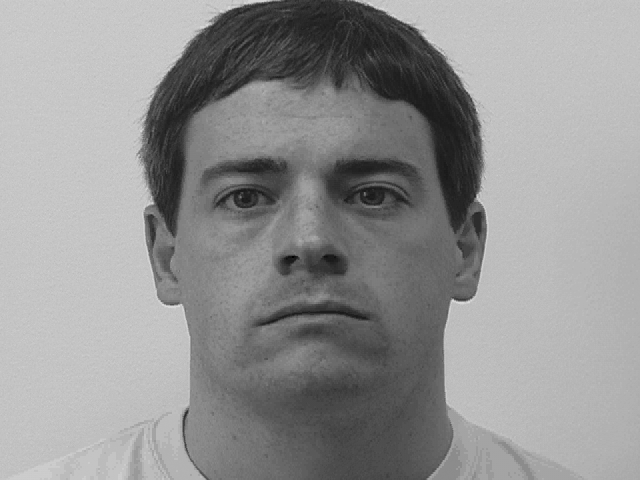
\includegraphics[width=\textwidth]{./img/dataset/neutral.png}
		\caption{neutral}
		\label{fig:dataset:neutral}
	\end{subfigure}
	%\hspace{\fill}
	\begin{subfigure}[b]{0.22\textwidth}
		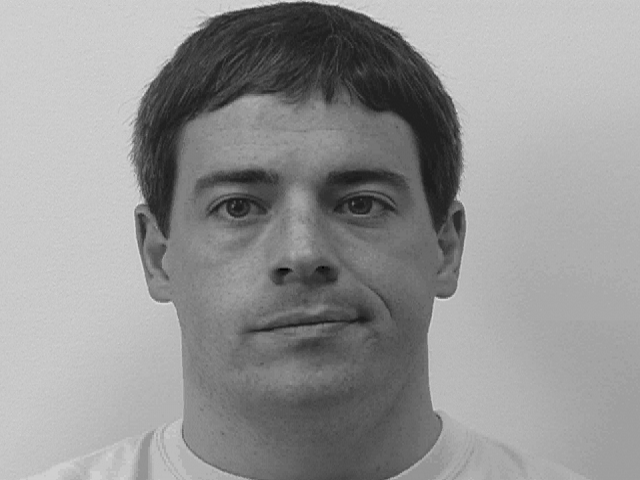
\includegraphics[width=\textwidth]{./img/dataset/contempt.png}
		\caption{contempt}
		\label{fig:dataset:contempt}
	\end{subfigure}
%\hspace{\fill}
	\begin{subfigure}[b]{0.22\textwidth}
		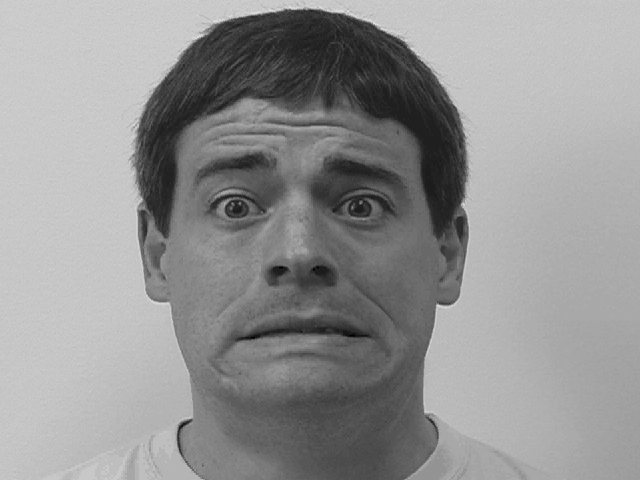
\includegraphics[width=\textwidth]{./img/dataset/fear.png}
		\caption{fear}
		\label{fig:dataset:fear}
	\end{subfigure}
%\hspace{\fill}
	\begin{subfigure}[b]{0.22\textwidth}
		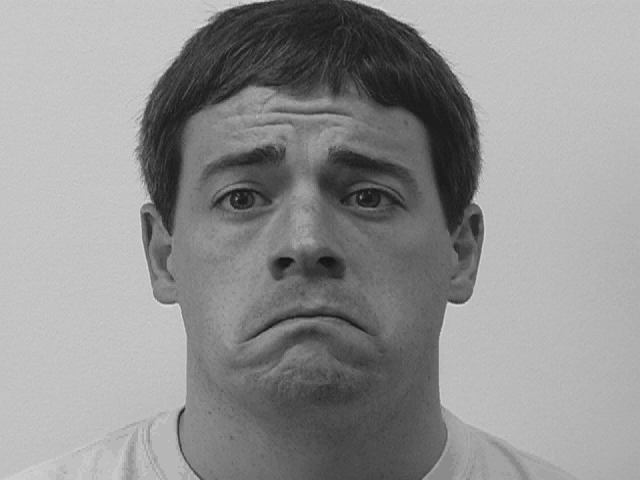
\includegraphics[width=\textwidth]{./img/dataset/sadness.png}
		\caption{sadness}
		\label{fig:dataset:sadness}
	\end{subfigure}
%\hspace{\fill}
	\begin{subfigure}[b]{0.22\textwidth}
		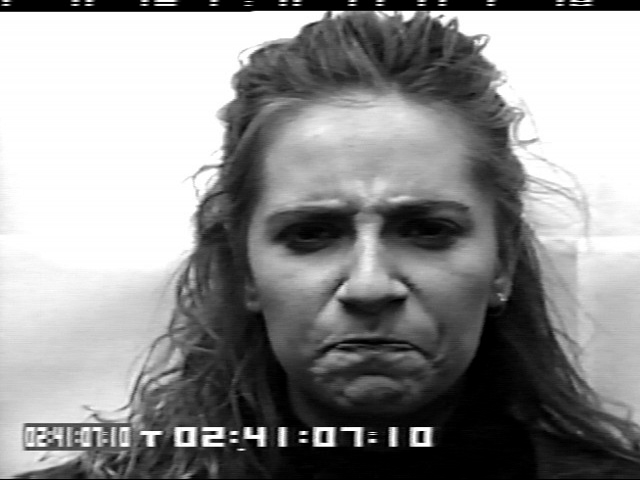
\includegraphics[width=\textwidth]{./img/dataset/angry.png}
		\caption{angry}
		\label{fig:dataset:angry}
	\end{subfigure}
%\hspace{\fill}
	\begin{subfigure}[b]{0.22\textwidth}
		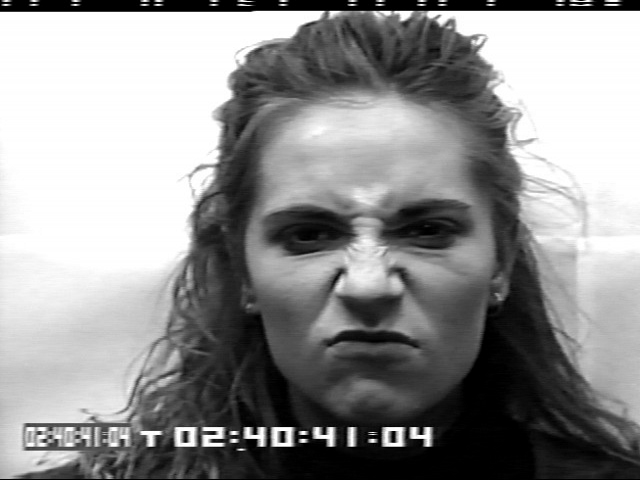
\includegraphics[width=\textwidth]{./img/dataset/disgust.png}
		\caption{disgust}
		\label{fig:dataset:disgust}
	\end{subfigure}
%\hspace{\fill}
	\begin{subfigure}[b]{0.22\textwidth}
		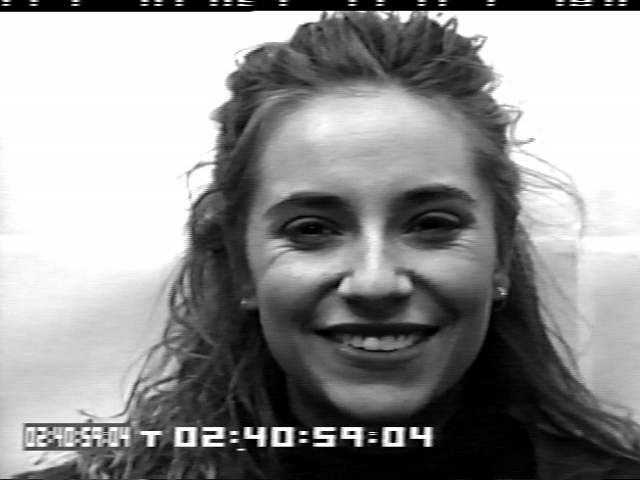
\includegraphics[width=\textwidth]{./img/dataset/happy.png}
		\caption{happy}
		\label{fig:dataset:happy}
	\end{subfigure}
%\hspace{\fill}
	\begin{subfigure}[b]{0.22\textwidth}
		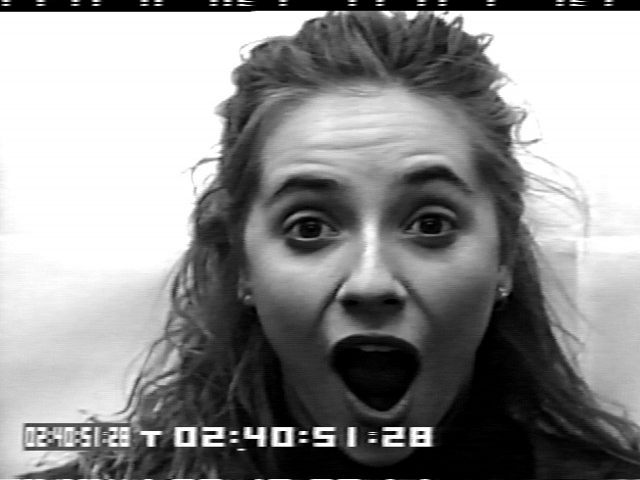
\includegraphics[width=\textwidth]{./img/dataset/surprise.png}
		\caption{surprise}
		\label{fig:dataset:surprise}
	\end{subfigure}
    \caption[Examples of intense facial expressions]{Examples of intense facial expressions from two subjects in the dataset}
    \label{fig:dataset images}
\end{figure}

\subsection{Manually Extracted Patches}\label{sec:data:manual}

An image can have multiple discriminating patches. As shown in Figure \ref{fig:manual_patch}, some patches are highly and noticeably discriminating such as an open mouth and raised eyebrows in "`surprise"' expression or a wrinkled glabella (area between eyes) in "`disgust"' expression. Such patches can be the best approximation of most discriminating patches. Hence, they make a good basis for testing the algorithm.

\begin{figure}
\centering
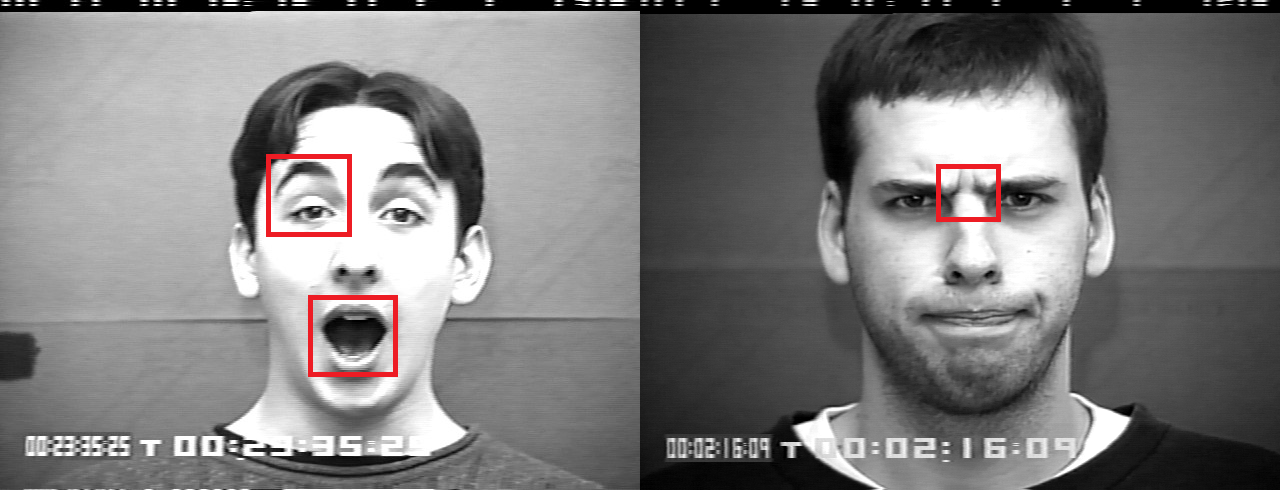
\includegraphics[width=200pt]{img/manual_patch.png}
  \caption{Noticeably discriminating patches}
  \label{fig:manual_patch}
\end{figure}

According to the approach described by \cite{Singh2012DiscPat}, such patches should be discovered and clustered in an unsupervised way using the k-means algorithm. However, due to problems encountered with the very large number of possible patches per image and time constraints it was decided to identify the most noticeably discriminating patches manually. We identified four such patches, two patches for eyes and one each for the mouth and the glabella. We extracted them manually and it was ensured that extracted images of same patch are consistent with each other in terms feature content of the patch. For example, in case of mouth patches, it was ensured that the boundaries of the patch touch the edges of lips in all mouth patches. It is very important that the patches are consistent and optimal otherwise the results can be poor. This is reflected from Table \ref{table:predict_unaliged_surprise} and Table \ref{table:predict_unaliged_fear} in the section 4.5.


These manually extracted patches were rescaled to 36*36 pixels, 64*64 pixels and 96*96 pixels. Tables \ref{table:left_eye}, \ref{table:right_eye}, \ref{table:between_eyes} and \ref{table:mouth} show the results for each region, for classifiers trained with the patch size of 96*96 , 32*32 and 64*64 pixels. Shrinking the images on the one hand results in fewer HOG features which is likely to reduce the effect of overfitting, on the other hand some visual information may be lost. The table entries represent the fraction of the images of the corresponding expression that were correctly classified.

